% -*- TeX -*- -*- UK -*-
% ----------------------------------------------------------------
% arXiv Paper ************************************************
%
% Subhaneil Lahiri's template
%
% Before submitting:
%    Comment out hyperref
%    Comment out showkeys
%    Replace \newcommand{\mlim}[2]{{\stackrel{\scriptstyle #1}{#2}}}
\newcommand{\ra}{\rightarrow}
\newcommand{\lr}{\leftrightarrow}
\newcommand{\cdt}{\!\cdot\!}
\newcommand{\vp}{\vspace{0.5cm}}
\newcommand{\degs}{^\circ}
%
%e.g., i.e. with normal spaces
\newcommand{\eg}{e.g.\ }
\newcommand{\ie}{i.e.\ }
\newcommand{\cf}{cf.\ }
\newcommand{\etc}{etc.\ }
%
% indices
\newcommand{\up}[1]{\mbox{}^{#1}}
\newcommand{\dn}[1]{\mbox{}_{#1}}
\newcommand{\rp}[1]{^{(#1)}}
\newcommand{\lp}[1]{_{(#1)}}
%
% brackets etc.
\newcommand{\prn}[1]{\left ( #1 \right )}
\newcommand{\brc}[1]{\left\{ #1 \right\}}
\newcommand{\brk}[1]{\left [ #1 \right ]}
\newcommand{\abs}[1]{\left\lvert #1 \right\rvert}
\newcommand{\nrm}[1]{\left\lVert #1 \right\rVert}
\newcommand{\av}[1]{\left\langle #1 \right\rangle}
%
% QM Dirac notation
\newcommand{\bra}[1]{\left\langle #1 \right \rvert}
\newcommand{\ket}[1]{\left \lvert #1 \right\rangle}
\newcommand{\braket}[2]{\left\langle #1 \midddle | #2 \right\rangle}
\newcommand{\bracket}[3]{\left\langle #1 \middle | #2 \middle | #3 \right\rangle}
%
% Derivatives, etc. First argument is optional.
\newcommand{\diff}[3][\rule{0mm}{0mm}]{\frac{\mathrm{d}^{#1} #2}{\mathrm{d}{#3}^{#1}}}
\newcommand{\pdiff}[3][\rule{0mm}{0mm}]{\frac{\partial^{#1} #2}{\partial {#3}^{#1}}}
\newcommand{\pdiffc}[3][\rule{0mm}{0mm}]{\left (\frac{\partial #2}{\partial {#3}}\right )_{\!\!#1}}
\newcommand{\pdl}[1][\rule{0mm}{0mm}]{\overleftarrow{\partial}_{#1}}
\newcommand{\pdr}[1][\rule{0mm}{0mm}]{\overrightarrow{\partial}_{#1}}
\newcommand{\pdlr}[1][\rule{0mm}{0mm}]{\overleftrightarrow{\partial_{#1}}}
\newcommand{\fdf}[2]{\frac{\delta #1}{\delta #2}}
\newcommand{\intd}[1]{\int\!\dr #1\,}
%
% Un-italicised letters
\newcommand{\dr}{\mathrm{d}}
\newcommand{\e}{\mathrm{e}}
\newcommand{\ir}{\mathrm{i}}
\DeclareMathOperator{\tr}{tr}
\DeclareMathOperator{\Tr}{Tr}
\DeclareMathOperator{\Det}{Det}
%
% The default \Im and \Re look crap
\renewcommand{\Im}{\operatorname{\mathfrak{Im}}}
\renewcommand{\Re}{\operatorname{\mathfrak{Re}}}
%
% Referencing sections, figures, etc
\newcommand{\sref}[1]{\S\ref{#1}}
\newcommand{\cref}[1]{Ch.\ref{#1}}
\newcommand{\Cref}[1]{Ch.\ref{#1}}
\newcommand{\fref}[1]{fig.\ref{#1}}
\newcommand{\Fref}[1]{Fig.\ref{#1}}
\newcommand{\tref}[1]{tab.\ref{#1}}
\newcommand{\Tref}[1]{Tab.\ref{#1}}
%
\newcommand{\nn}{\nonumber}
%
% Put the preprint numbers in the top right corner of the page.
% Use after \maketitle.
% First argument: How high it needs to be raised,
% Second argument: Width of the box,
% Third argument: The preprint numbers.
\newcommand{\preprintno}[3]{\hfill\raisebox{#1}[0cm][0cm]{
\begin{minipage}[t]{#2}\begin{flushright} #3 \end{flushright}\end{minipage}}
\vspace*{-\baselinestretch\baselineskip}}
%
% If you have changed the line spacing, e.g. with \renewcommand{\baselinestretch}{1.5},
% the command \sgap produces a line break with the normal spacing.
\newlength{\lingap}
\setlength{\lingap}{\baselinestretch\baselineskip}
\addtolength{\lingap}{-\baselineskip}
\newcommand{\sgap}{\\[-\lingap]}
 with its contents
%       or include mydefs.tex in zip/tar file
%    Replace %
\newcommand{\CD}{\mathcal{D}}
\newcommand{\CE}{\mathcal{E}}
\newcommand{\CG}{\mathcal{G}}
\newcommand{\CH}{\mathcal{H}}
\newcommand{\CK}{\mathcal{K}}
\newcommand{\CO}{\mathcal{O}}
\newcommand{\CL}{\mathcal{L}}
\newcommand{\CM}{\mathcal{M}}
\newcommand{\CN}{\mathcal{N}}
\newcommand{\CV}{\mathcal{V}}
\newcommand{\CZ}{\mathcal{Z}}
%
\newcommand{\dM}{\mathfrak{M}}
\newcommand{\dmd}{\mathfrak{d}}
\newcommand{\dmD}{\mathfrak{D}}
%
\newcommand{\R}{\mathbb{R}}
\newcommand{\C}{\mathbb{C}}
\newcommand{\CP}{\mathbb{CP}}
\newcommand{\Z}{\mathbb{Z}}
%
\newcommand{\ad}{{\dot{\alpha}}}
\newcommand{\bd}{{\dot{\beta}}}
\newcommand{\gd}{{\dot{\gamma}}}
\newcommand{\dd}{{\dot{\delta}}}
\newcommand{\ed}{{\dot{\epsilon}}}
%
\newcommand{\bs}{\overline{\sigma}}
\newcommand{\br}{\overline{\rho}}
\newcommand{\bpsi}{\overline{\psi}}
\newcommand{\bchi}{\overline{\chi}}
\newcommand{\bPsi}{\overline{\Psi}}
\newcommand{\bQ}{\overline{Q}}
\newcommand{\bS}{\overline{S}}
\newcommand{\bJ}{\overline{J}}
\newcommand{\zb}{{\bar z}}
\newcommand{\wb}{{\overline w}}
\newcommand{\cb}{{\bar c}}
\newcommand{\ab}{{\bar a}}
\newcommand{\bb}{{\bar b}}
\newcommand{\bp}{{\bar\partial}}
%
\newcommand{\p}{\partial}
\newcommand{\apm}{{\alpha^{\prime}}}
\newcommand{\adg}{a^\dagger}
\newcommand{\psq}{^{\prime\,2}}
\newcommand{\ppsq}{^{\prime\prime\,2}}
\newcommand{\half}{\frac{1}{2}}
%
 with its contents
%       or include newsymb.tex in zip/tar file
%    Put this file, the .bbl file, any picture or
%       other additional files and natbib.sty
%       file in a zip/tar file
%
% **** -----------------------------------------------------------
\documentclass[12pt]{article}
% Preamble:
%\usepackage{a4wide}
\usepackage[centertags]{amsmath}
%\usepackage{ams} for finding documentation only
\usepackage{amssymb}
%\usepackage{amsthm}
\usepackage[sort&compress,numbers]{natbib}
%\usepackage{citeB}
\usepackage{ifpdf}
\usepackage{graphicx}
%\usepackage{graphics} for finding documentation only
%\usepackage{xcolor}
%\usepackage{pgf}
\graphicspath{{figs/}}
\usepackage{adjustbox}
\newcommand{\aligntop}[1]{\adjustbox{valign=t}{#1}}
\usepackage{epstopdf}
\epstopdfsetup{update,suffix=-generated}
\ifpdf
 \usepackage[pdftex,bookmarks,bookmarksopen,pdfstartview=FitH]{hyperref}
 \epstopdfDeclareGraphicsRule{.svg}{pdf}{.pdf}{%
 "C:/Program Files (x86)/Inkscape/inkscape" -f #1 -D -A \OutputFile
 }
\else
 \usepackage[hypertex]{hyperref}
 %\DeclareGraphicsRule{.png}{eps}{.bb}{}
\fi
%
\usepackage{paralist}
\newenvironment{myenuma}{\begin{inparaenum}[(a)]}{\end{inparaenum}}
\newenvironment{myenumi}{\begin{inparaenum}[(i)]}{\end{inparaenum}}
\newenvironment{myenumA}{\begin{inparaenum}[\bfseries A.]}{\end{inparaenum}}
\newenvironment{myenumI}{\begin{inparaenum}[\bfseries I.]}{\end{inparaenum}}
%
% >> Only for drafts! <<
\usepackage[notref,notcite]{showkeys}
% ----------------------------------------------------------------
\vfuzz2pt % Don't report over-full v-boxes if over-edge is small
\hfuzz2pt % Don't report over-full h-boxes if over-edge is small
%\numberwithin{equation}{section}
%\renewcommand{\baselinestretch}{1.5}
% ----------------------------------------------------------------
% New commands etc.
\newcommand{\mlim}[2]{{\stackrel{\scriptstyle #1}{#2}}}
\newcommand{\ra}{\rightarrow}
\newcommand{\lr}{\leftrightarrow}
\newcommand{\cdt}{\!\cdot\!}
\newcommand{\vp}{\vspace{0.5cm}}
\newcommand{\degs}{^\circ}
%
%e.g., i.e. with normal spaces
\newcommand{\eg}{e.g.\ }
\newcommand{\ie}{i.e.\ }
\newcommand{\cf}{cf.\ }
\newcommand{\etc}{etc.\ }
%
% indices
\newcommand{\up}[1]{\mbox{}^{#1}}
\newcommand{\dn}[1]{\mbox{}_{#1}}
\newcommand{\rp}[1]{^{(#1)}}
\newcommand{\lp}[1]{_{(#1)}}
%
% brackets etc.
\newcommand{\prn}[1]{\left ( #1 \right )}
\newcommand{\brc}[1]{\left\{ #1 \right\}}
\newcommand{\brk}[1]{\left [ #1 \right ]}
\newcommand{\abs}[1]{\left\lvert #1 \right\rvert}
\newcommand{\nrm}[1]{\left\lVert #1 \right\rVert}
\newcommand{\av}[1]{\left\langle #1 \right\rangle}
%
% QM Dirac notation
\newcommand{\bra}[1]{\left\langle #1 \right \rvert}
\newcommand{\ket}[1]{\left \lvert #1 \right\rangle}
\newcommand{\braket}[2]{\left\langle #1 \midddle | #2 \right\rangle}
\newcommand{\bracket}[3]{\left\langle #1 \middle | #2 \middle | #3 \right\rangle}
%
% Derivatives, etc. First argument is optional.
\newcommand{\diff}[3][\rule{0mm}{0mm}]{\frac{\mathrm{d}^{#1} #2}{\mathrm{d}{#3}^{#1}}}
\newcommand{\pdiff}[3][\rule{0mm}{0mm}]{\frac{\partial^{#1} #2}{\partial {#3}^{#1}}}
\newcommand{\pdiffc}[3][\rule{0mm}{0mm}]{\left (\frac{\partial #2}{\partial {#3}}\right )_{\!\!#1}}
\newcommand{\pdl}[1][\rule{0mm}{0mm}]{\overleftarrow{\partial}_{#1}}
\newcommand{\pdr}[1][\rule{0mm}{0mm}]{\overrightarrow{\partial}_{#1}}
\newcommand{\pdlr}[1][\rule{0mm}{0mm}]{\overleftrightarrow{\partial_{#1}}}
\newcommand{\fdf}[2]{\frac{\delta #1}{\delta #2}}
\newcommand{\intd}[1]{\int\!\dr #1\,}
%
% Un-italicised letters
\newcommand{\dr}{\mathrm{d}}
\newcommand{\e}{\mathrm{e}}
\newcommand{\ir}{\mathrm{i}}
\DeclareMathOperator{\tr}{tr}
\DeclareMathOperator{\Tr}{Tr}
\DeclareMathOperator{\Det}{Det}
%
% The default \Im and \Re look crap
\renewcommand{\Im}{\operatorname{\mathfrak{Im}}}
\renewcommand{\Re}{\operatorname{\mathfrak{Re}}}
%
% Referencing sections, figures, etc
\newcommand{\sref}[1]{\S\ref{#1}}
\newcommand{\cref}[1]{Ch.\ref{#1}}
\newcommand{\Cref}[1]{Ch.\ref{#1}}
\newcommand{\fref}[1]{fig.\ref{#1}}
\newcommand{\Fref}[1]{Fig.\ref{#1}}
\newcommand{\tref}[1]{tab.\ref{#1}}
\newcommand{\Tref}[1]{Tab.\ref{#1}}
%
\newcommand{\nn}{\nonumber}
%
% Put the preprint numbers in the top right corner of the page.
% Use after \maketitle.
% First argument: How high it needs to be raised,
% Second argument: Width of the box,
% Third argument: The preprint numbers.
\newcommand{\preprintno}[3]{\hfill\raisebox{#1}[0cm][0cm]{
\begin{minipage}[t]{#2}\begin{flushright} #3 \end{flushright}\end{minipage}}
\vspace*{-\baselinestretch\baselineskip}}
%
% If you have changed the line spacing, e.g. with \renewcommand{\baselinestretch}{1.5},
% the command \sgap produces a line break with the normal spacing.
\newlength{\lingap}
\setlength{\lingap}{\baselinestretch\baselineskip}
\addtolength{\lingap}{-\baselineskip}
\newcommand{\sgap}{\\[-\lingap]}

%
\newcommand{\CD}{\mathcal{D}}
\newcommand{\CE}{\mathcal{E}}
\newcommand{\CG}{\mathcal{G}}
\newcommand{\CH}{\mathcal{H}}
\newcommand{\CK}{\mathcal{K}}
\newcommand{\CO}{\mathcal{O}}
\newcommand{\CL}{\mathcal{L}}
\newcommand{\CM}{\mathcal{M}}
\newcommand{\CN}{\mathcal{N}}
\newcommand{\CV}{\mathcal{V}}
\newcommand{\CZ}{\mathcal{Z}}
%
\newcommand{\dM}{\mathfrak{M}}
\newcommand{\dmd}{\mathfrak{d}}
\newcommand{\dmD}{\mathfrak{D}}
%
\newcommand{\R}{\mathbb{R}}
\newcommand{\C}{\mathbb{C}}
\newcommand{\CP}{\mathbb{CP}}
\newcommand{\Z}{\mathbb{Z}}
%
\newcommand{\ad}{{\dot{\alpha}}}
\newcommand{\bd}{{\dot{\beta}}}
\newcommand{\gd}{{\dot{\gamma}}}
\newcommand{\dd}{{\dot{\delta}}}
\newcommand{\ed}{{\dot{\epsilon}}}
%
\newcommand{\bs}{\overline{\sigma}}
\newcommand{\br}{\overline{\rho}}
\newcommand{\bpsi}{\overline{\psi}}
\newcommand{\bchi}{\overline{\chi}}
\newcommand{\bPsi}{\overline{\Psi}}
\newcommand{\bQ}{\overline{Q}}
\newcommand{\bS}{\overline{S}}
\newcommand{\bJ}{\overline{J}}
\newcommand{\zb}{{\bar z}}
\newcommand{\wb}{{\overline w}}
\newcommand{\cb}{{\bar c}}
\newcommand{\ab}{{\bar a}}
\newcommand{\bb}{{\bar b}}
\newcommand{\bp}{{\bar\partial}}
%
\newcommand{\p}{\partial}
\newcommand{\apm}{{\alpha^{\prime}}}
\newcommand{\adg}{a^\dagger}
\newcommand{\psq}{^{\prime\,2}}
\newcommand{\ppsq}{^{\prime\prime\,2}}
\newcommand{\half}{\frac{1}{2}}
%

%matrices
\newcommand{\inv}{^{-1}}
\newcommand{\dg}{^\dagger}
\newcommand{\trans}{^\mathrm{T}}
\newcommand{\I}{\mathbf{I}}
\newcommand{\omb}{\overline{\omega}}
% ----------------------------------------------------------------
%
%%%%%%%%%%%%%%%%%%%%%%%%%%%%%%%%%%%%%%%%%%%%%%%%%%%%%%%%%%%%%%%%%%%%%%%%%%
% Title info:
\title{Illusions of criticality in high-dimensional autoregressive models}
%
% Author List:
%
\author{Subhaneil Lahiri and Surya Ganguli
%
}

\begin{document}

\maketitle


%%%%%%%%%%%%%%%%%%%%%%%%%%%%%%%%%%%%%%%%%%%%%%%%%%%%%%%%%%%%%%%%%%%%%%%%%%


\begin{abstract}
  We look at the eigenvalue spectrum of high-dimensional autoregressive models when applied to white-noise.
\end{abstract}

\tableofcontents

%%%%%%%%%%%%%%%%%%%%%%%%%%%%%%%%%%%%%%%%%%%%%%%%%%%%%%%%%%%%%%%%%%%%%%%%%%
% Beginning of Article:
%%%%%%%%%%%%%%%%%%%%%%%%%%%%%%%%%%%%%%%%%%%%%%%%%%%%%%%%%%%%%%%%%%%%%%%%%%

\section{The problem}\label{sec:theprob}

Consider a model of the following type
%
\begin{equation}\label{eq:model}
  x(t+1) = A x(t) + \text{noise},
\end{equation}
%
where $x(t)$ is an $N$-element vector and $A$ is an $N\times N$ matrix.

Suppose we have a sample of $P$ consecutive times, so $x$ is an $N\times P$ matrix.
We can perform a least-squares estimate of $A$ by minimising
%
\begin{equation}\label{eq:minL}
  L = \half\sum_{i,\mu} \prn{ x_{i\mu+1} - \sum_j A_{ij} x_{j\mu} }^2 = \half\Tr \prn{xU-Ax}\prn{xU-Ax}\trans,
\end{equation}
%
where $U$ is a shift matrix.
It will be useful to use periodic boundary conditions in time, \ie $x_{iP+1}\sim x_{i1}$,
as this will make $U$ orthogonal:
%
\begin{equation}\label{eq:Udef}
  U_{\mu\nu} = \delta_{\mu\nu+1} + \delta_{\mu1}\delta_{\nu P}.
\end{equation}
%
The estimate of $A$ is then
%
\begin{equation}\label{eq:Aest}
  A = \prn{xUx\trans}\prn{xx\trans}\inv.
\end{equation}
%

Suppose we attempted this analysis in a situation where there really is no structure,
\ie when $x(t)$ is white noise.
Then the true optimal $A$ would be 0.
However, with finite $P$ the estimate \eqref{eq:Aest} will not be zero.

We will look at the average eigenvalue distribution:
%
\begin{equation}\label{eq:eigdist}
  \rho(\omega) = \av{\rho_A(\omega)}_x,
  \qquad
  \rho_A = \sum_{i=1}^N \delta(\omega-\lambda_i),
\end{equation}
%
where $\lambda_i$ are the eigenvalues of $A$ in \eqref{eq:Aest} and
the components of $x$ are iid gaussian random variables with mean 0 and variance 1.

Following \cite{Sommers1988asymmetric}, this can be computed from a potential:
%
\begin{equation}\label{eq:potential}
  \rho_A(\omega) = -\nabla^2 \Phi_A(\omega),
  \qquad
  \Phi_A(\omega) = -\frac{1}{4\pi N} \ln\det \brk{(\omb-A\trans)(\omega-A)}.
\end{equation}
%
We define a partition function
%
\begin{equation}\label{eq:partfn}
  \Phi_A(\omega) = \frac{1}{4\pi N} \ln Z_A(\omega),
  \qquad
  Z_A(\omega) = \det \brk{(\omb-A\trans)(\omega-A)}\inv.
\end{equation}
%
The problem is now to compute $\av{\ln Z_A(\omega)}_z$.

%\subsection*{Acknowledgements}


%%%%%%%%%%%%%%%%%%%%%%%%%%%%%%%%%%%%%%%%%%%%%%%%%%%%%%%%%%%%%%%%%%%%%%%%%
\subsection*{Appendices}
\appendix
%%%%%%%%%%%%%%%%%%%%%%%%%%%%%%%%%%%%%%%%%%%%%%%%%%%%%%%%%%%%%%%%%%%%%%%%%

\section{Complex Gaussian integrals}\label{sec:compgauss}

First, Let's get all of the factors of 2 straight.
Note that if we write $z=x+\ir y$, then $\dz\dzb = 2\dx\dy$.
Let $H$ be a positive-definite, $N\times N$ Hermitian matrix.
Consider an integral  of the form
%
\begin{equation*}
  \int \prn{\prod_i\dz_i\dzb_i} \exp\prn{-z\dg H z}.
\end{equation*}
%
We can diagonalise $H$ with a unitary change of variables:
%
\begin{equation}\label{eq:compgausint}
\begin{aligned}
  \int \prn{\prod_i\dz_i\dzb_i} \exp\prn{-z\dg H z} &=
    \prod_i \int \dz_i\dzb_i\, \exp\prn{-\lambda_i \abs{z_i}^2} \\
    &= \prod_i \int \dx_i\dy_i\, 2\exp\prn{-\lambda_i \prn{x_i^2+y_i^2}} \\
    &= \prod_i \frac{2\pi}{\lambda_i}\\
    &= \frac{(2\pi)^N}{\det H}.
\end{aligned}
\end{equation}
%

The proper normalisation for a gaussian distribution is
%
\begin{equation}\label{eq:compgaussnorm}
  P(z,z\dg)\dz\dz\dg = \prn{\prod_i\frac{\dz_i\dzb_i}{2\pi}} \frac{\exp\prn{-z\dg C\inv z}}{\det C}.
\end{equation}
%
By completing the square, we can see that
%
\begin{equation}\label{eq:compgausslin}
  \av{\exp\prn{\zeta\dg z + z\dg\zeta}} = \exp\prn{\zeta\dg C\zeta}.
\end{equation}
%
Taking partial derivatives \wrt $\zeta_i$ and $\bar{\zeta}_i$, we find
%
\begin{equation}\label{eq:compgauscov}
  \av{zz\dg} = C.
\end{equation}
%

Now consider an integral of the form
%
\begin{equation}\label{eq:compgaussquad}
\begin{aligned}
  \av{\exp\prn{-z\dg A z}} &=
    \int \prn{\prod_i\frac{\dz_i\dzb_i}{2\pi}}\frac{\exp\prn{-z\dg (C\inv+A) z}}{\det C} \\
    &= \prn{\det C\det\prn{C\inv+A}}\inv \\
    &= \det\prn{I+CA}\inv.
\end{aligned}
\end{equation}
%


\section{Contour integrals for determinants}\label{sec:contourints}

In evaluating determinants, we will come across contour integrals of the form
%
\begin{equation}\label{eq:contourint}
  I(z) = \frac{1}{2\pi\ir}\int \frac{\dr\zeta}{\zeta} \ln(z-\zeta),
\end{equation}
%
where the contour is the unit circle in a counter-clockwise direction.
The contour might not be closed because of the branch cut.
We choose the branch of the logarithm so that
%
\begin{equation}\label{eq:branch}
  \arg\prn{\frac{\zeta-z}{z}} \in [0,2\pi],
\end{equation}
%
and we define $\theta=\arg z$. The branch cut is shown in \fref{fig:contours}.

\begin{figure}
 \begin{center}
 \begin{myenuma}
  \item\aligntop{\includegraphics[width=5cm]{contout.svg}}\label{fig:contout}
  \hspace{1cm}
  \item\aligntop{\includegraphics[width=5cm]{contin.svg}}\label{fig:contin}
 \end{myenuma}
 \end{center}
  \caption{Contours used to evaluate \eqref{eq:contourint}, (\ref{fig:contout}) when $\abs{z}>1$, (\ref{fig:contin}) when $\abs{z}<1$.}\label{fig:contours}
\end{figure}

If $\abs{z}>1$, we can use the contour $C_1$ in \fref{fig:contours}(\ref{fig:contout}).
Using the residue theorem:
%
\begin{equation}\label{eq:intout}
  I(z) = \frac{1}{2\pi\ir}\int_{C_1} \frac{\dr\zeta}{\zeta} \ln(z-\zeta) = \ln z.
\end{equation}
%

If $\abs{z}>1$, we can use the contour $C_2$ in \fref{fig:contours}(\ref{fig:contin}):
%
\begin{equation}\label{eq:contout}
C_2: \quad
  \begin{aligned}
    \zeta &= \e^{\ir\phi},                             & \phi &\in [\theta+\delta,\theta+2\pi-\delta], \\
    \zeta &= \e^{\ir(\theta+2\pi-\delta)}+xz\prn{1-\e^{\ir(2\pi-\delta)}},
                                                       & x    &\in [0,1], \\
    \zeta &= z - x \e^{\ir(\theta+2\pi-\delta)}, \quad & x    &\in [\abs{z}-1,-\epsilon], \\
    \zeta &= z + \epsilon\e^{-\ir\phi},                & \phi &\in [-\theta-2\pi+\delta,-\theta-\delta], \\
    \zeta &= z + x \e^{\ir(\theta+\delta)},          & x    &\in [\epsilon,1-\abs{z}.] \\
    \zeta &= \e^{\ir(\theta+\delta)}+(1-x)z\prn{1-\e^{\ir\delta}},
                                                       & x    &\in [0,1], \\
  \end{aligned}
\end{equation}
%
Using the residue theorem:
%
\begin{equation}\label{eq:intin}
  \frac{1}{2\pi\ir}\int_{C_2} \frac{\dr\zeta}{\zeta} \ln(z-\zeta) = \ln z.
\end{equation}
%
If we let $\delta,\epsilon\to0$, the second, fourth and sixth parts of the contour integral vanish, and the first part gives $I(z)$ in \eqref{eq:contourint}.
We're left with
%
\begin{equation}\label{eq:intinlim}
  \begin{aligned}
    \ln z &= I(z)
           -\frac{1}{2\pi\ir} \int_{\abs{z}-1}^{0} \frac{\e^{\ir\theta}\dx}{z-x\e^{\ir\theta}} \ln\prn{x\e^{\ir(\theta+2\pi)}}
           +\frac{1}{2\pi\ir} \int_{0}^{1-\abs{z}} \frac{\e^{\ir\theta}\dx}{z+x\e^{\ir\theta}} \ln\prn{-x\e^{\ir\theta}}  \\
      &= I(z)
           -\frac{1}{2\pi\ir} \int_{0}^{1-\abs{z}} \frac{\dx}{\abs{z}+x} \ln\prn{-x\e^{\ir(\theta+2\pi)}}
           +\frac{1}{2\pi\ir} \int_{0}^{1-\abs{z}} \frac{\dx}{\abs{z}+x} \ln\prn{-x\e^{\ir\theta}}  \\
      &= I(z) - \int_{0}^{1-\abs{z}} \frac{\dx}{\abs{z}+x}  \\
      &= I(z) + \ln\abs{z}.
  \end{aligned}
\end{equation}
%

Therefore:
%
\begin{equation}\label{eq:countourintresult}
  I(z) = \frac{1}{2\pi\ir}\int \frac{\dr\zeta}{\zeta} \ln(z-\zeta) = \ln z - [\ln\abs{z}]_-,
\end{equation}
%
where $[x]_\pm = x \theta(\pm x)$ and $\theta(x)$ is the Heaviside step function.


\section{The quadratic function $\Gamma(\zeta)$}\label{sec:Gamma}








%%%%%%%%%%%%%%%%%%%%%%%%%%%%%%%%%%%%%%%%%%%%%%%%%%%%%%%%%%%%%%%%%%%%%%%%%%

\bibliographystyle{utcaps_sl}
\bibliography{maths,qft,neuro}

\end{document}
